\documentclass[a4paper, 11pt]{article}

\usepackage{comment} % enables the use of multi-line comments (\ifx \fi)
\usepackage{lipsum} %This package just generates Lorem Ipsum filler text.
\usepackage{fullpage} % changes the margin
\usepackage{hyperref}

% \usepackage[backend=bibtex,style=verbose-trad2]{biblatex}
%\usepackage[backend=bibtex,
%  bibencoding=utf8
%  ]{biblatex}
% \usepackage[style=numeric-comp,natbib=true,backend=bibtex,bibencoding=utf8]{biblatex}
% \AtEveryBibitem{%
%   \clearfield{issn} % Remove issn
%   \clearfield{doi} % Remove doi
%   \clearfield{eprint} % Remove eprint
%   \clearfield{pages} % Remove pages number
%
%   \ifentrytype{online}{}{% Remove url except for @online
%     \clearfield{url}
%   }
% }
%\addbibresource{bib/mybib}
\usepackage{subcaption}
% \usepackage{subfig}
\usepackage{wrapfig}
\usepackage{xfrac}
\usepackage{multirow}
\usepackage{empheq}
\usepackage{mathtools}
\usepackage[sc]{mathpazo}
\usepackage{float}
\usepackage[dvipsnames, table]{xcolor}

\usepackage{tabu}
\usepackage{longtable}

\usepackage{graphicx}
\usepackage{caption}
\captionsetup{%
  font=small,% set font size to footnotesize
  labelfont=bf % bold label (e.g., Figure 3.2) font
}
\captionsetup[sub]{font=footnotesize,labelfont={bf,sf}}
\usepackage{array,booktabs}
\usepackage{framed}

\usepackage{amsmath}

\usepackage{pgfplots}        % make nice plots using raw data
\usepgfplotslibrary{external}
\usepackage{pstricks,pst-plot,psfrag}% Post-script graphics
\usetikzlibrary{plotmarks}
\usepackage{textcomp}
\usetikzlibrary{shapes,arrows}
 %define plots
\pgfplotsset{
  /pgfplots/xlabel near ticks/.style={
    /pgfplots/every axis x label/.style={
      at={(ticklabel cs:0.5)},anchor=near ticklabel
    }
  },
  /pgfplots/ylabel near ticks/.style={
    /pgfplots/every axis y label/.style={
      at={(ticklabel cs:0.5)},rotate=90,anchor=near ticklabel
    }
  }
}
\pgfplotsset{compat=newest}
\pgfplotsset{plot coordinates/math parser=false}

\usepackage{pgfgantt}

\setcounter{secnumdepth}{3} % only chapter and sections will be numbered
\setcounter{tocdepth}{1}    % entries down to \subsubsections in the TOC

\usepackage{enumitem}
%\usepackage{fouriernc}
% \usepackage{indentfirst}  % Causes the document to indent the first paragraph after a section
\usepackage{tabularx}
\usepackage{todonotes}
\usepackage{pdfpages}


%%%%%%%%%%%%%%%%%%%% Color definitions %%%%%%%%%%%%%%%%%%%%%

\definecolor{aaublue}{RGB}{33,26,82}

\definecolor{tableHeader}{RGB}{211, 47, 47}
\definecolor{tableLineOne}{RGB}{245, 245, 245}
\definecolor{tableLineTwo}{RGB}{224, 224, 224}

\definecolor{bulletColor}{HTML}{323642}


%%%%%%%%%%%%%%%%%%%% New Commands %%%%%%%%%%%%%%%%%%%%%%%%%%%
\newcommand{\tableHeaderStyle}{
    \rowfont{\leavevmode\color{white}\bfseries}
    \rowcolor{tableHeader}
}
\newcommand{\degree}{$^\circ$}
\newcommand{\micrometer}{$\mu$m}

% Black square bullets within lists
\newcommand{\localtextbulletone}{\textcolor{bulletColor}{\raisebox{.2ex}{\rule{1.0ex}{1.0ex}}}}
\renewcommand{\labelitemi}{\localtextbulletone}
\newcommand{\degreeC}{$^{\circ}$C}

% Table style definition
\taburowcolors[2] 2{tableLineOne .. tableLineTwo}
\tabulinesep = ^2mm_1mm
\everyrow{\tabucline[.4mm  white]{}}


\begin{document}
%Header-Make sure you update this information!!!!
%\noindent
%\large\textbf{Post/Pre-Lab X Report} \hfill \textbf{FirstName LastName} \\
%\normalsize ECE 100-003 \hfill Teammates: Student1, Student2 \\
%Prof. Oruklu \hfill Lab Date: XX/XX/XX \\
%TA: Adam Sumner \hfill Due Date: XX/XX/XX

\tableofcontents
\newpage
\section{Name of Candidate and Provisional Thesis Title}\label{sec:name_title}
\begin{itemize}
  \item[] \textbf{Candidate Name:} \texttt{Sean \textsc{Thomas} }
  \item[] \textbf{Provisional Thesis Title:} \texttt{Smart Grippers: Conception of a novel type of \\
  actuator powered by Shape Memory Alloys}
\end{itemize}

\section{Keywords}\label{sec:keywords}
Shape Memory Alloy, Buckled Beam, NiTiNOL, Shape Memory Effect, Bistable system, Self-switching, Modelling and Optimization, Printed Electronics

\section{Research Field and Motivation}\label{sec:research_mot}
\subsection{Motivation}\label{subsec:motivation}
%
% Currently, the Mikron workshops are equipped with pneumatic grippers, the Schunk MPG-25 as shown in figure 1. This type of gripper is currently the best of the market with an excellent power to weight ratio. But the force provided by the gripper is too high by a factor of 10 compared to the needs of the company. With the cheapest version of the MPG-25 series, it is necessary to pass two nozzles of the air injection monitor, next to the moving part of the robot, to the gripper, thus complexifying the design of the arms compared to a power supply. Furthermore, any pneumatic installation requires an air pump. In general, the capacity of the latter depends on the number of grippers used at the same time. When the number of active grippers drops, the pump always runs at the same speed, resulting in a loss of efficiency. The last critical point of this technology is its adaptation in a clean environment. Since these grippers release a certain amount of air during each change of position. It is imperative to install a high-quality air filter that will have to be changed regularly to ensure that the installation complies with the cleanliness standards in some areas such as biomedical.
%
% On the market, there are a wide variety of gripper that use different gripping techniques. Some operate using air suction, which creates a pressure difference under a tube and acts like a suction cup to grip objects. They are particularly useful for flat and smooth objects. Due to the low flexibility with regards to the type of parts that can be handled, these types of grippers are not very widespread. In the same manner, there are electromagnetic grippers where magnetic parts are manipulated. These grippers can be sized specifically to serve different sizes of pieces.
%
% Shape memory alloys (SMA) are alloys that have the particular property of not respecting the Hooke’s law with respect to deformation. The material possesses two distinctive phases, the Austenite and Martensite phases. The temperatures at which the material transforms into the two phases are known as the Austenite and Martensite temperature. By heating the material above this temperature, it is possible, after plastic deformation, to bring it back to its initial position. Furthermore, this position can be precisely chosen.
%
% In order to have a system allowing Mikron SA to maximise the rate of their assembly, we focused on optimizing the weight of the proposed actuator. By comparing the response times obtained by some laboratories, including MIT with electrically heated SMAs, we decided to actuate using thin SMA blades. We plan to differentiate ourselves from traditional SMA actuators by developing a hybrid heating solution that combines internal Joule effect heating and an external heater. We propose that this would significantly reduce the transition time of the SMA and optimize the time response. We also decided to use a mobile magnet to increase the efficiency and performance of the actuator as illustrated in Figure 6 in the annex. On either side of the actuator, we intend to place ferromagnetic pieces which will attract the magnet with the certain amount of force. This setup will give us the two stable positions required. A mechanism with several NiTiNOL blades will deform when the magnet arrives and these blades will be used to alternate between the two stable positions by applying the initial force to actuate the magnet. By heating the blades, the SMA will change phase and their stiffness will increase causing it to apply a force onto the magnet. Once this force exceeds the attractive force of the magnet, the mobile magnet will be attracted and be displaced to the other stable position on the opposite side. There are have been multiple studies into SMAs, such as [1], that show that SMAs have a very high power to weight ratio when compared to other types of actuation. The proposed mechanism allows us to match the product requirements while at the same time being extremely lightweight.
%
%  Moreover, as suggesting in [3], in order to have a sufficient lifecycle, the maximum deformation of the material should not exceed 3\%. We have decided to dedicate a work package for this critical area of the project. There are have been some research that looks into different methods by which SMA blades can be heated and cooled such as [4]. Using printed coils and passing an electric current, we can use the Joule effect to effectively heat the blade. By extensively studying different heating and cooling solutions, we can hope to obtain an optimized solution that would allow us to mitigate this risk.
In an era where manual assembly is no longer possible in the majority of developed countries, it is necessary for companies offering alternative solutions to stand out from their competitors. Manufacturers of assembly lines must modify the capabilities of their robots in order to be as competitive as possible compared to the relocation of the assembly in countries with cheaper labour. In order to stand out, companies such as Mikron SA, seek to increase the efficiency of their installations while preserving the precision appreciated by their customers. The goal of this project would be to conceive and develop a novel and innovative type of Smart gripper. This small part plays a primordial role in the dynamics of the robot. Being at the end of the arm, a small gain in weight of this part would have great consequences on the acceleration and the maximum speed that the robot will be able to reach.

The \emph{Laboratory of Integrated Actuators}, along with a Swiss company, \emph{Mikron SA}, intend to develop a novel type of gripper that will harness the high work output per volume of Shape Memory Alloys (SMA). This gripper would be designed to be lightweight and compact so as to be used as a pick and place gripper in clean room application. The project strives to create an innovative technology that will exploit the characteristics of this smart material to create an actuator that is highly responsive, dynamic, lightweight and compact. These objective will motivate a doctoral thesis that is challenging and innovative.

\subsection{Research Field}\label{subsec:research_field}
This project will focus on high response SMA actuation with a large stroke. Currently, few industrial actuators based on SMAs have been seen. This project first has to demonstrate the potential of such actuators as a gripper. Then optimisation of the right topology should reveal the full potential of SMA actuators in terms of time response and stroke. Heating the element is not the greatest challenge, the cooling time of the material must also be taken into account. It is important to note that it is often harder to dissipate heat rather than accumulate it. Thus, various heating and cooling solutions will be exploited and investigated during this project. Another challenge to overcome would be the limited fatigue life of such smart materials. The gripper should at the very least have a fatigue life in the order of $10^6$ cycles. The last challenge to over overcome would be to meet the requirements set by the currently used pneumatic grippers in industry.

This investigation will consider the thermal and mechanical aspect of the material so as to create a highly responsive and dynamic actuator capable of achieving the required force output of traditional grippers. The main focus of the research will be the thermal and mechanical optimization. The conception of the gripper will include optimization of the geometrical topology of the SMA blades and the use of bistable systems such as buckled beams to create dynamic and high stroke actuators. The command strategies of the actuator will also be an important area of study due to the fact that the actuation of the SMA will involve the precise control of its temperature and resistance.

The symbiosis of the bistable system and the SMA technology can result in an innovative gripper system. The interplay between these two domains will be studied and explored in this thesis.

\subsection{Specifications}\label{subsec:specifications}
The specifications of the actuator were obtained by comparing it with the specifications of the Schunk MPG-25 which is the most common pneumatic gripper used in industry, more specifically the primary gripper used by Mikron SA.

\begin{table}[H]%{r}{5.5\textwidth}
  \centering
  \footnotesize
  \caption{Specifications of the required actuator}
  \label{tab:specs}
  \begin{tabu} to 0.5\textwidth {>{\bfseries}X[l, 3]  >{\bfseries}X[l, 1] X[r,1]}
      \tableHeaderStyle{tableRed}
      Criteria & Units & Value\\
      Stroke & mm & 3\\
      Grip force & N & 5\\
      Commutation time & ms & 50 - 100\\
      Weight & g & 100\\
      Precision/Repeatability & mm & 0.02\\
      Number of stable positions & \# & 2\\
      Volume & mm$^3$ & 120 \\
  \end{tabu}
\end{table}

Using the above specifications, the energy that the smart material must supply can be calculated to be approximately 15 mJ. This implies, for example, that for materials such as SMAs, the application would require only a volume of 1.5 mm$^3$.
% The \emph{Laboratoire d'actionneurs int\'{e}gr\'{e}s} (LAI), along an international NGO and two Swiss companies, are developing a novel suit concept that will be paired with a high-reliability ventilation system. This protective suit is designed to \emph{refresh} and \emph{protect} professionals of the health sector, who battle infectious diseases in tropical climates and in remote areas of developing countries. This context induces high constraints in terms of harsh working environment, limited maintenance possibilities, and financial resources.
%
% The cooperation strives to develop a suit that is portable, robust and economically accessible. Its ventilation system and its corresponding drive, complying with the aforementioned characteristics, will motivate a doctoral thesis at the \emph{EPFL}. To this end, a miniaturized electric drive with magnetics bearings seems suitable for the constraining operating conditions, given its close-to-none maintenance needs, construction simplicity and thus their miniaturization potential.
% \subsection{Research Field}\label{subsec:research_field}
% This investigation will focus upon high-speed rotatory electric drives and magnetic bearings. It will also exhibit an industrial profile, since it is aspires to set the cornerstones of new product trends of its supporting companies.
%
% Therefore, this projects considers the conception, construction, and commissioning of a \emph{magnetically levitated }(mag-lev) motor. The correct deliberation of practical and theoretical aspects will determine the success of this research.
%
% For the conception, one of the supporting companies will define what type of ventilator topology is needed for the proper refreshing inside suit.  The selection of motor topology has to match ventilator geometry and its needed performance. The design of mag-lev drives diverges from classical motor design, since not only drive but \emph{bearing performance} has to be considered. On top, drive and bearing performance usually trade-off with one another, so an optimum has to be found.
%
% This conception has to consider the feasibility of actual manufacturing procedures.  The assembly of the drive will be challenging because the mechanical tolerances of manufacturing methods may be relatively large for the desired \emph{millimetric-scale} of the prototype. Homogenously-cut mechanical pieces, thin impeller elements and evenly-spaced sensor placement are crucial for the match between theory and the practice.
%
% Commissioning is the culmination of the conception and construction. It will involve read-in of various electric signals, its processing, and the generation of actuator commands, all at a digital level. Given that the motor will rotate at high-speeds, the code must be time-optimized. Various closed-loop plants will have to be tuned, for speed, rotor position and current control, and non-idealities will also have to be compensated for.
% \subsection{Specifications}\label{subsec:specs}
% To generate a scientific breakthrough, and simultaneously comply with the industrial requirements, the motor needs to meet the following requirements.
% \begin{center}
% \begin{tabular}{c|c|c|c}
%   % after \\: \hline or \cline{col1-col2} \cline{col3-col4} ...
%   Mass & Power & Rotational Speed & Axial length \\ \hline
%   $< 150$ g & $<30$ W & $> 100$ krpm & $< 50$ mm \\
% \end{tabular}
% \end{center}

\section{State of the Art : Smart Materials and Devices} \label{sec:sota}
This section will discuss the existing smart materials that are currently studied and used in the domain of actuators. The different techniques and integration systems will also be presented with the goal to compare the various approaches currently used.

% \subsection{Smart materials} \label{subsec:Smartmaterials}
In the field of engineering, there has been a need  to create actuators that are lightweight, compact and having force output. This creates a need for materials that can deliver high forces and strokes while remaining light and small meaning that the materials need to have a high work output.

On the basis of creating an actuator that can meet the demands of the currently implemented strategies while at the same time pushing the limits of the current technology, a thorough investigation of the available smart materials must be conducted. These materials have the ability to react mechanically to an external stimulus such as thermal electrical or magnetic and are thus referred to as \emph{smart} or \emph{active materials}. There exist numerous types of smart materials and based on their properties, they can be classified into many types based on their activation methods\cite{damodharan_review_2018}.
% \begin{itemize}
% 	\item Piezoelectric materials
% 	\item Magneto-strictive materials
% 	\item Electro-active polymers
% 	\item Shape Memory Alloys
% \end{itemize}

The system that incorporates the material is equally critical for the conception of the actuator. This section of the report will delved into different strategies used to harness the specific behaviours of the smart materials and integrate them into actuators.

\subsection{Piezoelectric Materials}
Piezoelectric materials like PZT are a well known type of smart material that reacts to voltages. These materials are already commercially available in various different gripper systems. The company PI is a supplier of PZT actuators such as the \href{https://www.physikinstrumente.com/en/products/piezoceramic-actuators/linear-actuators/p-604-compact-piezomove-linear-actuator-202820/}{P-604 Compact PiezoMove Linear} actuator and many more such suppliers already exist.

\begin{wrapfigure}{r}{0.45\textwidth}
	\centering
	\vspace{-10pt}
	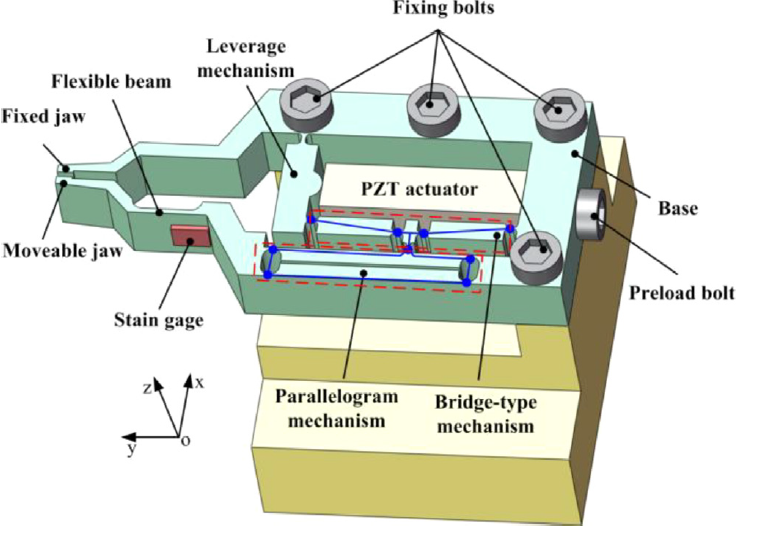
\includegraphics[width=0.40\textwidth]{Figures/PZT_grip.png}
	\caption{Mechanism of the PZT gripper\cite{liang_design_2018}.}
	\vspace{-10pt}
	\label{fig:PZT_grip}
\end{wrapfigure}

PZT actuators are widely used due to the fact that they have small volumes, high output force ($\sim10^5$ J/m$^3$) and fast response times (10$^6$ Hz)\cite{faran_ferromagnetic_2016}. But generally these materials have quite a small maximum stroke, generally around 20 \micrometer for a 0.5 mm stack\cite{rupitsch_piezoelectric_2019}. This implies that PZT actuators will require the integration of amplifiers that will increase the total displacement of the actuator. The work performed by Liang et al., 2018\cite{liang_design_2018} displays a micro-gripper that is comprised of a PZT along with an integrated amplifying system as shown in figure \ref{fig:PZT_grip}. The study uses flexure-based mechanical structures as an amplifier so as to create a high stroke gripper without a great increase in the total volume of the gripper.

An interested approach to designing the amplification system has been observed in the study performed by Ruiz and Sigmund, 2018\cite{ruiz_optimal_2018}. In this work, a large displacement PZT microgripper was designed from a rectangular plate using topology optimization. Here, the PZT plate is sandwiched between two electrodes and an input voltage is applied. This voltage will generate an electric field and will create a deformation in the PZT structure. The optimisation strategy is to increase the deformation by varying the shape and dimensions of the total structure. This strategy could be used in not just this instance but to optimize the actuation of any actuator built around an active smart material.

Based on the literature and the specifications of the gripper, the volume of the piezoeletric material required to fulfil the 15 mJ of work can be calculated to be 150 mm$^3$.

\subsection{Electro-Active polymers}
Electroactive Polymers (EAP) have the ability to alter their mechanical behaviour such as a change in shape or size when exposed to an electric field. EAPs emerged in the last few decades exhibiting large strains when exposed to electrical stimulus \cite{bar-cohen_artificial_2005}.

\begin{wrapfigure}{l}{0.45\textwidth}
	\centering
	\vspace{-5pt}
	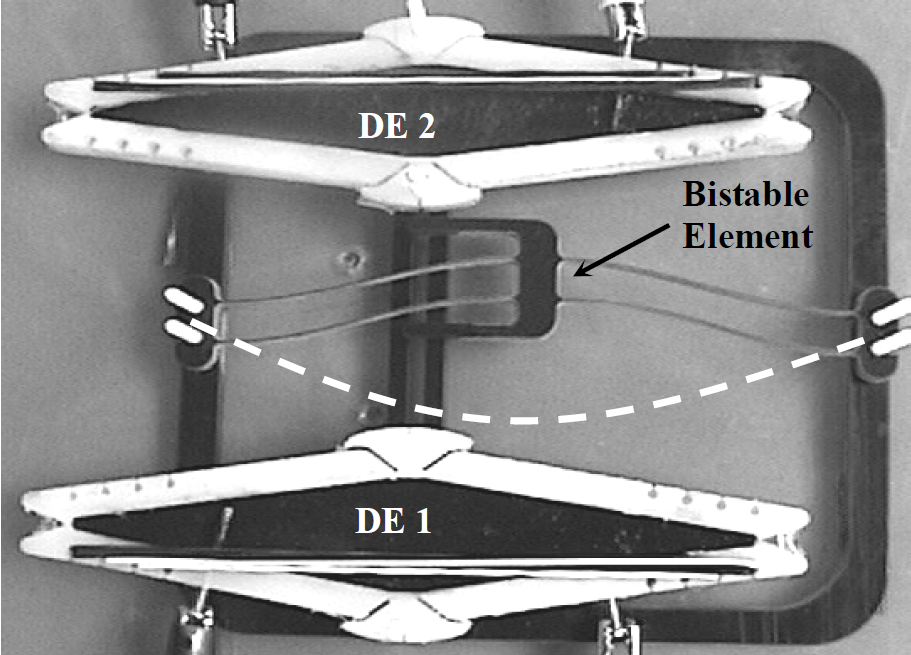
\includegraphics[width=0.4\textwidth]{Figures/DEAP_flipflop.png}
	\caption{DEAP Flip-flop bistable actuator concept\cite{plante_compliant_2005}.}
	\vspace{-10pt}
	\label{fig:DEAP_flipflop}
\end{wrapfigure}

EAP can generate high strains, with Dielectric elastomers (DE) such as silicone exhibiting strains of about 63\%\cite{kornbluh_electroactive_2004}. EAP materials can also exhibit greater response times, in the order of 10$^5$ Hz, when compared to smart materials such as shape memory alloys, which will be explored in the next section. EAP can be very useful for their fast actuation times, low density and greater resilience and can, thus, be very convenient when create mechanical devices that are light weight and compact.

The behaviour of the film is caused by the interaction of the electrostatic charges that are created on the opposing electrodes. By applying a voltage on the two electrodes, the electrodes are subjected to opposite charges cause an attractive force between them.

\textbf{Dielectric Electro-Active Polymer} (DEAP) actuators are comprised of an elastomeric film that is platted on both sides with a compliant electrode as shown in figure.The system is actuated when a high voltage is applied between the two electrodes.The main drawback of using DEAP actuators are the fact that they have very small fatigue life which is around $10^3$ cycles\cite{chen_preliminary_2017}. By attempting to use the DEAP actuators in a continuous fashion, it will result in a short lifetimes and low reliability. In the paper written by Plante et al,. 2005\cite{plante_properties_2007,chouinard_bistable_2012} as seen in figure \ref{fig:DEAP_flipflop} or by Wang et al., 2018\cite{wang_design_2018}, the teams overcome the burdens of short fatigue life by coupling the DEAP actuator with a bistable element. Here, the work displays DEAP actuators and a flip-flop bistable mechanism, where two agonistic-antagonistic actuators move a buckled beam back and forth. The DEAP actuator works as an external trigger mechanism that, when actuated, will force the bistable element into its opposing stable state.

The work shows that the approach to use an antagonistic actuators with a smart material as a trigger mechanism are capable of approximately 10x greater volumetric energy density when compared to traditional flip-flop devices.

\begin{wrapfigure}{r}{0.4\textwidth}
	\centering
	\vspace{-10pt}
	
\includegraphics[width=0.35\textwidth]{Figures/IPMC_fig.eps}
	\caption{IPMC actuation principle\cite{poubel_proposal_2011}.}
	\vspace{-5pt}
	\label{fig:IPMC_act}
\end{wrapfigure}

\textbf{Ionic EAP} are another variant of EAPs which differ from the DEAP which are sometimes referred to as Electronic EAP\cite{bar-cohen_artificial_2005}. The difference between the two variants arises from the fact that the actuation in Ionic EAPs is a result of diffusion of ions. An interesting Ionic EAP material are Ionic polymer-metal composites (IPMC). These IPMCs are a type of synthetic composite material that has a muscle-like behaviour under an applied voltage or electric field. In figure \ref{fig:IPMC_act}, the working principle is shown where as a voltage is applied, the diffusion of ions within the material causes a deformation. They are generally ionic polymers that are chemically plated with conductors\cite{shahinpoor_ionic_1998}.

\begin{figure}[H]
    \centering
    \begin{subfigure}[t]{0.27\textwidth}
			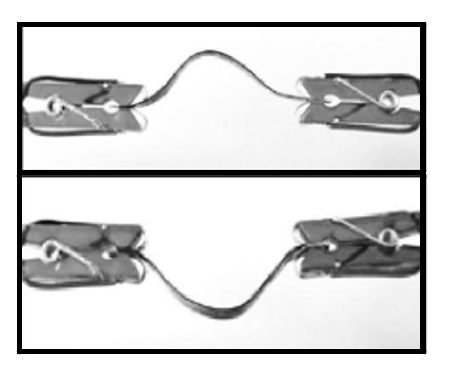
\includegraphics[width=\textwidth]{Figures/IPMC_buckle.eps}
			\caption{Nafion-based IPMC in the two buckled states.}
			\label{fig:IPMC_buckle}
    \end{subfigure}
		~
     %add desired spacing between images, e. g. ~, \quad, \qquad, \hfill etc.
      %(or a blank line to force the subfigure onto a new line)
    \begin{subfigure}[t]{0.6\textwidth}
			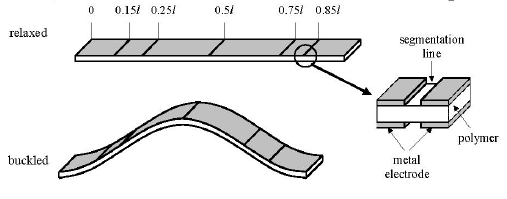
\includegraphics[width=\textwidth]{Figures/IPMC_segment.png}
			\caption{Segmentation at minimal static stress points.}
			\label{fig:IPMC_segment}
    \end{subfigure}
		\caption{Self-switching IPMC buckled beam\cite{rossiter_self-switching_2006}.}
		\label{fig:IPMC_work}
\end{figure}

IPMC bending actuators have been used primarily used as bending actuators and artificial muscles. A novel work conducted by Rossiter et al., 2006\cite{rossiter_self-switching_2006, rossiter_bistable_2006} where a self-switching strategy is explored within the scope of a buckled bistable beam made entirely of the IPMC smart material. The work addresses many disadvantages experienced by using a classical bistable buckled beam system with an external trigger mechanism such as relaxation after actuation, low repeatability and the need for energy to maintain the stable states. The work concludes that by use of self-switching system, where the material itself is used as the buckled monolithic beam and switches from one stable state to another using applied voltage, the aforementioned disadvantages can be addressed. In this work, a buckled monolithic IPMC beam is separated into a number of electrically independent segments. The work, then, proposes various strategies to activate the segments so as to actuate the beam into transitioning or bifurcating from one of the stable positions to another.

For the purpose of this project, as a means of comparison, the volume of the smart required was calculated. Based on the literature of the energy density and the 15 mJ of work obtained from specifications, the volume required was calculated to be about 20 mm$^3$ for silicone and about 500 mm$^3$ for IPMCs.

\subsection{Magneto-strictive materials}
The magneto-strictive materials have the ability to alter their mechanical behaviour and shape when subjected to magnetic fields. Magnetic Shape Memory Alloys (MSMA) are an interesting type of magneto-strictive material. Here, the MSMA shows an interesting behaviour in which the material when deformed will tend to remain stable and retain its deformed shape. As the materials is introduced into a strong magnetic field, the crystals of the material are realigned and the material reverts back to its predeformed shape. These MSMAs are an attractive choice as they are capable of high strains around 10\% while being able to prove fast response times in the order of 1 kHz\cite{faran_ferromagnetic_2016}.

The main drawbacks of MSMAs are the fact that they are quite a new technology implying that they are expensive and that finding suppliers is quite difficult. They are also quite brittle and are thus it makes it quite difficult to find them in different geometries and shapes.

The work presented by Gauthier et al., 2006\cite{gauthier_multistable_2006} details the fabrication of a multistable actuator that is based on these MSMAs. Here the device is a push-pull actuator with a pair of agonistic-antagonistic MSMA beams. The active material is actuated using magnetic fields that are created using coils and concentrated using ferromagnetic cores. In figure \ref{fig:MSMA_princ}, a working principle of the MSMA actuator can be seen.

\begin{wrapfigure}{r}{0.45\textwidth}
	\centering
	\vspace{-15pt}
	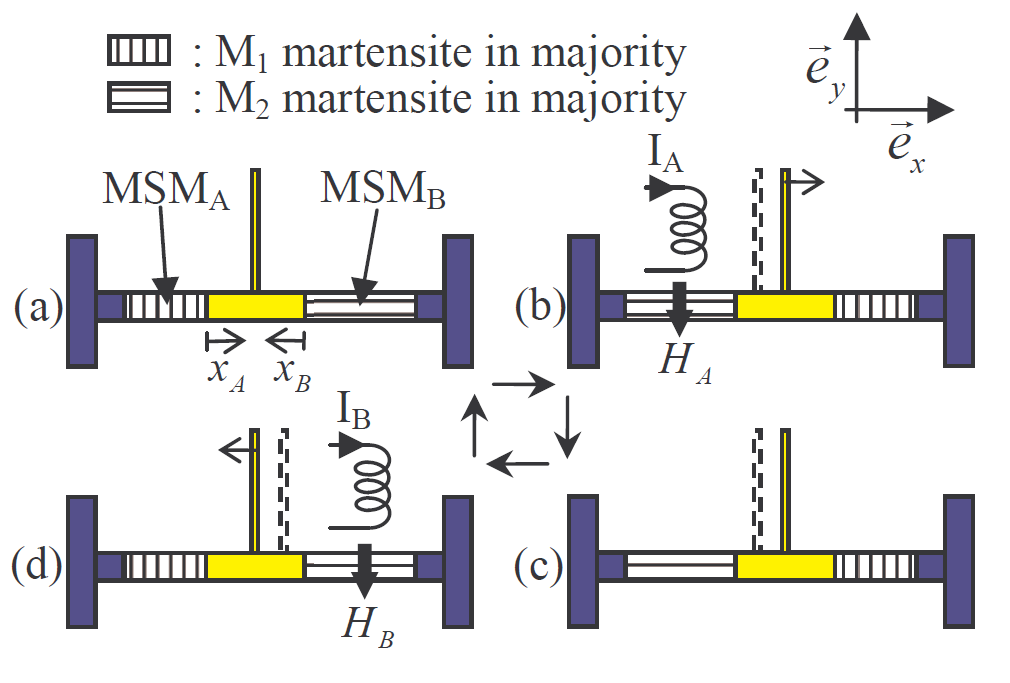
\includegraphics[width=0.4\textwidth]{Figures/MSMA_princ.png}
	\caption{Principle of the MSMA actuator\cite{gauthier_multistable_2006}.}
	\vspace{-10pt}
	\label{fig:MSMA_princ}
\end{wrapfigure}
The shape memory effect (SME) seen in the MSMA requires the material to be deformed before the application of the magnetic field. Only after the deformation can the strain recover of the SME be observed. In this work, the team was able to create a multistable actuator by using a pair of MSMA. Here, the activation of the first MSMA deformed the opposing beam and vice versa. This results in a displacement and positioning of an end effector placed in between the MSMAs. MSMAs as with traditional SMAs have to be deformed before any actuation can be observed. This work shows the advantages and breakthrough of using an agonistic-antagonistic pair of material to resolve the problem of having to predeform the active material.

One of the important factors that leads to this technology not being widely used, is the fact that the activation of the MSMA requires magnetic fields of around 0.6 T. The work by Lu at al., 2009\cite{lu_optimal_2009} shows the relationship between strain experienced by the material and the magnetic field density. The work shows an example of a differential rotating MSMA actuator that is powered using permanent magnets and ferromagnetic cores. This study shows that the limiting factor of these technology is the activation magnetic field required for the smart material. The resulting magnetic circuits will render the fabricated actuator to be heavy and bulky. In the use case presented in this work, a rough estimation of the dimensions of the magnetic circuit was established. A basic coil system with a volume of 6.3 cm$^3$ would be required to generate the 0.6 T needed for actuation. When compared to the 100 mm$^3$ of MSMA required to fulfil the 15mJ of work specified in the gripper specifications, the coil dimensions largely increased the total gripper volume. Thus, the MSMA material will ultimately be unsuitable for the use in small and light weight actuators as desired by this research.

\subsection{Shape Memory Alloys}
Shape memory alloys such NiTiNOL show two important properties: the Shape Memory Effect (SME) and Superelasticity (SE)\cite{rao_design_2015}. SMAs are a particular subgroup of smart materials that change their mechanical behaviour based on a thermal stimulus. Here, the material as with the MSMA, retains its shape when deformed and reverts back to its original shape when heated (SME). Shape Memory Alloys (SMA) actuators provide us with an opportunity to create such actuators due to their high work output per volume which is around 10 $\mathrm{J}/\mathrm{cm}^3$\cite{mohd_jani_review_2014}. This can be a 10-fold increase when compared to pneumatic actuators. The SMA actuators are thus able to provide large amounts of force when compared to their volume, making them particularly useful in compact, lightweight actuators.

SMAs are an attractive choice of material for the realisation of small and compact actuators due to their high energy density. They can provide high forces and displacements with a low volume of required material. However, they are thermally activated and have, thus, very long response times. Tomozawa et al.\cite{tomozawa2005}, 2005, have worked on fabricating a microactuator using thin film SMA with high transformation temperatures that work at a frequency of 100Hz. The high transformation temperatures and large surface area to volume ratio allows the SMA to cool down and achieve high frequencies. Vitushinsky et al.\cite{vitushinsky_bistable_2009}, 2009, have developed a highly responsive actuator by reducing the temperature hysteresis seen in SMAs using an actuator that is made up of two SMAs with different transition temperatures.

Paik and Wood\cite{paik_bidirectional_2012, paik_novel_2010}, 2012 devised a way to decrease the heating time of the SMAs by the way of printed-on coil. In this work, the actuator was fitted with a coil having a higher resistivity to further optimize the heating process by Joules heating. The use of an external heating element that was glued to the SMA has decreased the time response by around 30\%. Below is a simple heat exchange curve
\begin{equation}
	\label{eq:Tech}
	T(t) = (T_A - T_{\infty})e^{-t/\tau} + T_{\infty},~~\tau = \frac{C_m\rho V}{h s_{ech}}
\end{equation}
where $C_m$ is the specific heat capacity, $h$ is the heat transfer coefficient, $s_{ech}$ is the surface area of heat exchange, $V$ is the volume, $T_A$ is the austenitic finish temperature and $T_{\infty}$ is the ambient room temperature. This equation can be used to calculate the approximate time it would take to cool down the SMA material and thus determine the bandwidth of the material. Using 15 \micrometer~thick thin films or 25~\micrometer diameter thin wires and high temperature SMA (around $T_A$ = 90 \degreeC), the cooling time can be reduced to 20 ms.
A rough estimation of the required SMA for the gripper was calculated to be just around 1.5mm$^3$. Thus, a combination of the innovative ideas proposed in these above works can be used achieve effective results when designing a reactive and compact smart gripper.

\subsection{Comparison}
The aim of this section of the report is to find the most appropriate type of technology that can replace and innovate the current gripper that are employed in industry. In the current industrial era, most grippers employ the use of pneumatic actuators as their primary source of energy. Thus, to innovate the current domain of gripper, various important factors must be taken into account so as to have a point of comparison between the different smart materials and the presently used pneumatic grippers.

\begin{table}[h]
  \centering
	\footnotesize
  \caption{Comparison of smart material performances}
  \label{tab:comparison}
  \begin{tabu} to 1\textwidth {X[l, 2] X[l, 0.75] X[l,0.75] X[l,1] X[l,1] X[l,1.25]}
			\tableHeaderStyle{tableBlue}
      Actuator type & Stress [MPa] & Strain [\%] & Efficiency [\%] & Bandwidth [Hz] & Volumetric Work [J/\cc]\\
      Pneumatic \cite{mohd_jani_review_2014} & 0.7 & 50 & 90 & 20 & 0.175\\
			NiTi SMA \cite{mohd_jani_review_2014, rizzello_overview_2017, faran_ferromagnetic_2016} & 200 & 10 & 3 & $10^2$ & 10\\
			PZT \cite{kornbluh_electroelastomers:_2002, faran_ferromagnetic_2016} & 110 & 0.1 & 90 & $10^6$ & 0.1\\
			MSMA \cite{rizzello_overview_2017, faran_ferromagnetic_2016, karaca_magnetic_2009} & 100 & 6 & 90 & $10^3$ & 0.15\\
			EAP \cite{kornbluh_electroelastomers:_2002, faran_ferromagnetic_2016, rizzello_overview_2017} & 3 & 60 & 90 & $10^5$ & 0.75\\
			% Human Muscle \cite{hollerbach_comparative_1992, tadesse_electroactive_2013} & 0.8 & 100 & 35 & 173 & 0.035\\
  \end{tabu}
\end{table}
\begin{wrapfigure}{r}{0.45\textwidth}
	\centering
	\vspace{-5pt}
	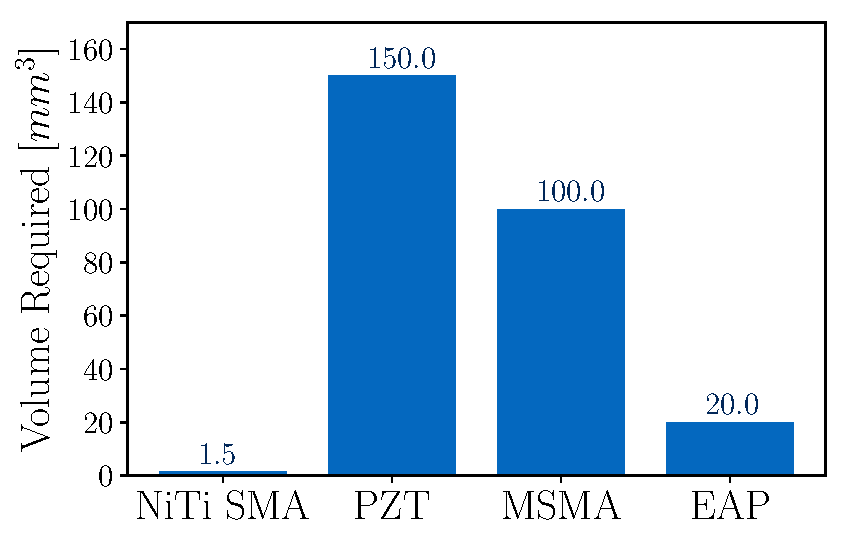
\includegraphics[width=0.4\textwidth]{Figures/Vol_Req_Bar.pdf}
	\vspace{-9pt}
	\caption{Approximate volume of the smart material required to fulfil the 15 mJ of work obtained from the gripper specifications.}
	% \vspace{-5pt}
	\label{fig:vol_req_bar}
\end{wrapfigure}
In the hopes of creating a compact and lightweight actuator, the most important parameter to consider would be the volumetric work. This parameters determines the level at which the active component of the actuator can be minimised when designing the gripper. The SMA offers a great deal better work output to volume ratio when compared to the other materials. The most critical aspect in this case would be attempting to optimize the time response of these SMA in hopes of improving a critical parameter in which this material is lacking.


% \begin{figure}[H]
% 	\centering
% 	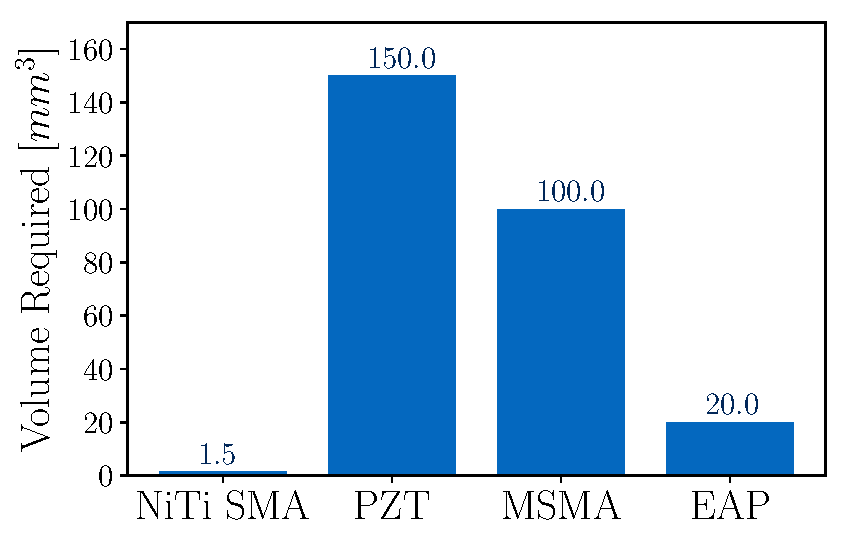
\includegraphics[width=0.4\textwidth]{Figures/Vol_Req_Bar.pdf}
% 	\caption{Approximate volume of the smart material required for the gripper based on the specifications and the volumetric work.}
% 	\label{fig:vol_req_bar}
% \end{figure}

\section{Work Accomplished}\label{sec:work_accomplished}
In the previous section, the state of the art explored the various ways in which literature shows the integration of smart materials in actuator systems. Bistable elements using buckled beams shows a lot of promise due to the fact that they do not require energy to maintain the stable position and their potential energy can be used to trigger fast and dynamic strokes.

\subsection{Finite Element Modelling of SMA}\label{ssec:WA_FEM}
SMAs exist in various different stable phases which consists of the \emph{Martensitic (M)} phase and the \emph{Austenitic (A)} phase. The M phase can exist in either the \emph{Twinned M} phase or the \emph{Detwinned M} phase based on the stress experienced by the material. When the material reaches the Austenic transformation temperature ($\mathbf{A_s}$) threshold, the material will begin to transform from the M phase to the A phase i.e. the Austenitic transformation. Inversely, as the material cools down to the Martensitic transformation temperature ($\mathbf{M_s}$), it will begin to transform from the A phase to the M phase i.e. the Martensitic transformation. Since these transformations occur over a range in temperature, we must heat and cool well beyond the transformation temperatures. The SMA that in most likelihood will be used is a type of NiTiNOL variant with a relatively high transformation temperature (with $A_s$ around 50\degreeC) and thus exists primarily in the M phase at room temperature.

Since the stress distribution in a buckled beam is inhomogeneous, a Finite Element Modelling (FEM) simulation is more suited to handle the complexity of the calculations. The FEM simulation is performed using the Shape Memory Effect material property found in ANSYS Workbench. Using the nine parameters defined in the material property toolbox, we can simulate the shape memory effect. These parameters were obtained by consulting the material properties established in literature and datasheets from manufacturers\cite{divringi_advanced_2009}.

 So as to ascertain the reliability of the shape memory effect model created using ANSYS, a simple elongation test was performed. ANSYS workbench was used to model a simple SMA blade and a tractional strain of 8$\%$ was applied. The figure \ref{fig:FigElongationStressStrain}, shows the evolution of the internal stress of the SMA blade during the ANSYS scenario. This elongation test allows us to create a uniform stressed SMA blade that will perform the same phase changes as seen in the more complex buckled SMA beam.

\begin{figure}[H]
 \centering
 \begin{subfigure}[t]{0.45\textwidth}
    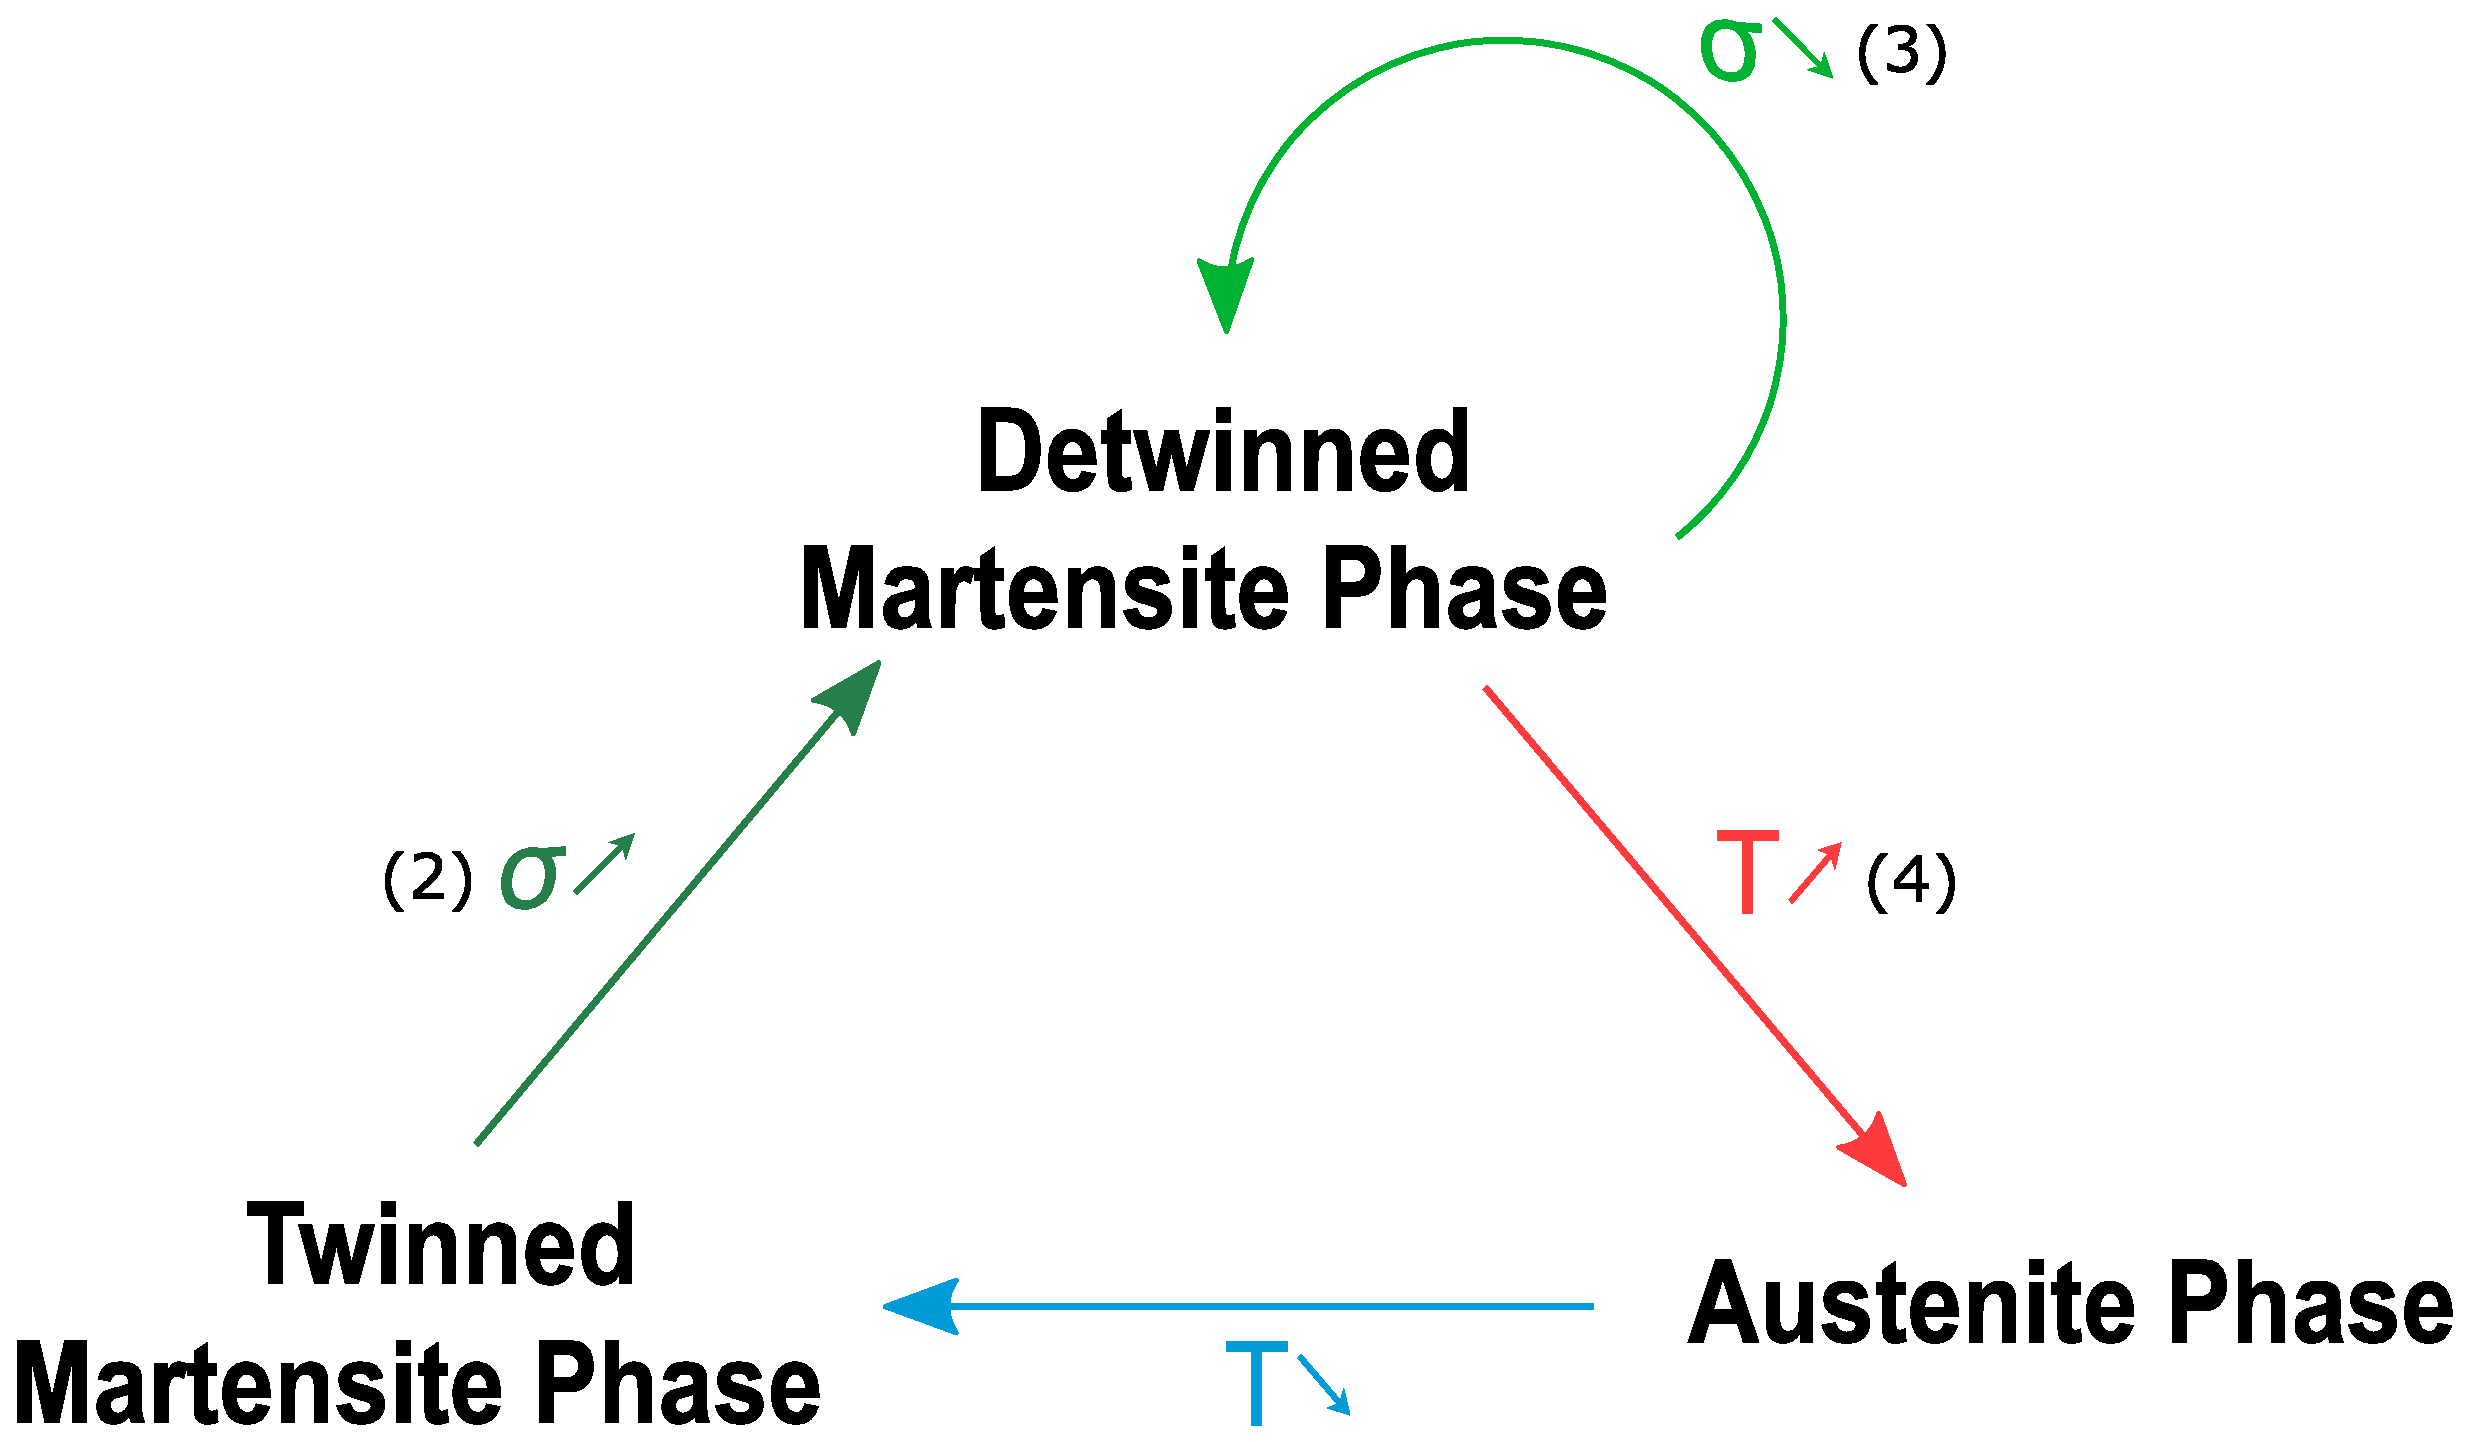
\includegraphics[width=\textwidth]{Figures/Phase_Transf_Diagram_Text.eps}
    \caption{Phase transformation diagram of a shape memory alloy. Here $\sigma$ represents the stress created by mechanical loading and T represents the temperature change due to thermal loading.}
    \label{fig:PhaseTransfDiagram}
 \end{subfigure}
	~
  %add desired spacing between images, e. g. ~, \quad, \qquad, \hfill etc.
   %(or a blank line to force the subfigure onto a new line)
 \begin{subfigure}[t]{0.45\textwidth}
    {\footnotesize
      \def\svgwidth{\textwidth}
      \input{Figures/FigElongationStressStrain.pdf_tex}
    }
    \vspace{-13pt}
    \caption{Finite element simulation of SMA Stress-Strain curve in traction and compression using a longitudinal bar}
    \label{fig:FigElongationStressStrain}
  \end{subfigure}
	\caption{The different phases and transformations of an SMA}
	\label{fig:SMAPhaseChange}
\end{figure}

The phase transformations can be seen in figure \ref{fig:PhaseTransfDiagram}. When a mechanical load is applied to the SMA while in its M phase, the material shears on an atomic level and this allows it to deform through a detwinning process at relatively low stress levels. This process allows the material to deform up to strains of 8$\%$. Strains larger than this will cause dislocations which are irreversible. In figure \ref{fig:FigElongationStressStrain}, we can see the various phase changes that occur within the SMA blade. Firstly, one end of the blade is fixed and the other end is subjected to a remote displacement so as to produce a strain. The resulting stress can be observed in region (1) of the figure. As the strain increases, the material reaches its stress threshold to transform from its twinned M phase to its detwinned M phase. This can be observed in region (2), where the strain increases rapidly. Once the blade has reached its maximal strain, the remote displacement is disabled. The region (3) shows that the blade loses its internal stress but remembers the deformation created by the mechanical load. Finally, the SMA blade is heated up and past its transformation temperature. This transforms the material from the A phase back to the M phase. This can be observed in region (4) where the graph shows the strain recovery of the material. This strain recovery is known as the Shape Memory Effect (SME). Thus, the strain of the material upon heating, immediately returns to zero and the elongation of the bar is recovered. This cycle can be observed in experimental tests studied in literature such as \cite{hongchun_xie_design_2007, liu_asymmetry_1998}

The FEM simulation was also used to ascertain the volumetric energy density of these SMA material. Here, again a simple monolithic beam was elongated and the work required for this elongation was estimated. Then, as the beam was heated above its transition temperature, the work output due to the strain recovery was measured. The difference between the two values allowed for the verification of the volumetric work presented by the literature shown in table \ref{tab:comparison}.

 % \begin{table}[H]
 % 	\centering
 % 	\footnotesize
 % 	\caption{SMA material property definitions}
 % 	\label{tab:matprop}
 % 	\begin{tabu} to 0.7\textwidth {X[l, 1.35] X[l, 0.65] X[r,3]}
 % 			\tableHeaderStyle{tableBlue}
 % 			\textbf{Property} & \textbf{Value} & \textbf{Definition} \\ [0.5ex]
 % 			$E_A$ [GPa] & 70 & Austenite Modulus \\
 % 			$E_M$ [GPa] & 30 & Martensite Modulus \\
 % 			$\nu$ & 0.3 & Poisson's Ratio \\
 % 			$H$ [GPa] & 1 & Hardening Parameter \\
 % 			$R$ [MPa] & 140 & Elastic Limit \\
 % 			$\beta$ [MPaK\textsuperscript{-1}] & 5.6 & Temperature Scaling Parameter \\
 % 			$T_0$ [K] & 323.15 & Reference Temperature \\
 % 			$\overline{\epsilon}_L$ [mm mm$^{-1}$] & 0.1 & Maximum Transformation Strain \\
 % 			$m$ & 0 & Lode Dependency Parameter \\
 % 	\end{tabu}
 % \end{table}

\subsection{Buckled beam modelling}
When a longitudinal monolithic beam is compressed and the critical axial load is reached, the beam will buckle and result in a bistable structure. The buckled beam will exist in two stable configurations as seen in the figure \ref{fig:States_Schema}. Specifically, this figure shows the two symmetrical stable states that the buckled beam can exist in for each given stable mode. The figure \ref{fig:Modes_Schema} shows the first three stable modes that are created when a longitudinal beam is pre-compressed.

\begin{figure}[H]
 \centering
 \begin{subfigure}[t]{0.45\textwidth}
   {\tiny
   \def\svgwidth{\textwidth}
   \input{Figures/BuckledBeamStable.pdf_tex}
   }
   \vspace{-10pt}
   \caption{Stable states of the buckled beam}
   \label{fig:States_Schema}
 \end{subfigure}
	~
  %add desired spacing between images, e. g. ~, \quad, \qquad, \hfill etc.
   %(or a blank line to force the subfigure onto a new line)
 \begin{subfigure}[t]{0.45\textwidth}
   {\tiny
   \def\svgwidth{\textwidth}
   \input{Figures/BuckledBeamModes.pdf_tex}
   }
   \vspace{-10pt}
   \caption{Diagram of the first three buckling modes}
   \label{fig:Modes_Schema}
  \end{subfigure}
	\caption{Representation of analytical model of buckled beam obtained from literature\cite{timoshenko_theory_1962}.}
	\label{fig:Buckled_Beam}
\end{figure}

When an axial load is applied to the longitudinal beam, the beam reaches a \emph{critical load} and is then deformed sideways, depending on the structure of the beam, to form one of the modes as seen in figure \ref{fig:Modes_Schema}.
% The modes can be described by the equation
% \begin{equation}
%   \label{eq:modeeq1}
%   \begin{split}
%     w = C\left(1-\cos\left(\frac{(j+1)\pi x}{l}\right)\right), \\
%     j = 1,3,5,...
%   \end{split}
% \end{equation}
% which describes the deflection for the odd modes where $C$ is an arbitrary constant, $l$ is the length of the beam and $x$ is the coordinate along the length of the beam. The equation
% \begin{equation}
%   \label{eq:modeeq2}
%   \begin{split}
%     w = C\Big[1-2\frac{x}{l}-\cos\left(k\frac{x}{l}\right) + \frac{2\sin(n_jx/l)}{n_j})\Big], \\
%     k = 2.86\pi, 4.92pi, 6.94\pi, 8.95\pi,...\quad j = 2,4,6,...
%   \end{split}
% \end{equation}
% describes the deflection of the even modes obtained from \cite{timoshenko_theory_1962}.
The figure \ref{fig:Modes_Schema} shows the two symmetric stables positions of the buckled beam. The beam can be triggered to switch from one of the states to the other by applying a vertical load at the apex of the curved beam. The displacement of the apex to a critical point will trigger the bifurcation or snap-through and thus the switching of states.

The modes seen in figure \ref{fig:Modes_Schema}, represent also the transition states of the beam as it transitions from one stable state to the opposing stable state \cite{rossiter_self-switching_2006}. When a vertical force is applied to the centre of the beam, the buckled beam is forced to transition to the third mode and then finally switches to the opposite state. While if a slight asymmetry is present in the fabrication of the beam or the actuation force, the beam transitions to the second state before switching to the opposite state.

Shape memory alloys can be used to create the buckled beam and can be used to supply the energy required to trigger the bifurcation. Since shape memory alloys can be activated using a thermal load, by applying a current through it, this allows the option to remove the central vertical force required and thus the external triggered required to trigger the switching. Thus, the SMA buckled beam actuation can be deemed a self-switching bistable mechanism. This paper will thus focus on the elimination of the external trigger in regards to standard bistable buckled beam actuators by using the potential energy stored within the SMA material.

\subsection{Self-switching of buckled SMA beam}
The next step of the research is to study the behaviour of a bistable buckled beam made entirely of an SMA. A monolithic beam of SMA is simulated and is then compressed from both ends to create the buckled beam as seen in figure \ref{fig:FigSMABlade}. The shape memory effect is only observed in areas of high stress where the material has exceeded the twinning threshold and has attained the twinned M phase as seen in figure \ref{fig:FigSMABlade}. Thus during the heating phase, these twinned M phase areas transform to the A phase and a vertical displacement of the apex of the buckled beam is observed. The goal of the research is to thus optimise the geometry so as to increase the maximum deformation of the buckled SMA beam when heated so as to create enough displacement that it will trigger bifurcation of the beam from one stable state to another. This behaviour can be deemed self-switching due to the fact that the system does not require an external trigger.

\begin{wrapfigure}{r}{0.45\textwidth}
	% \vspace{-5pt}
	\centering
  {\tiny
	\def\svgwidth{0.4\textwidth}
	\input{Figures/FigSMABlade3x_Edit.pdf_tex}
  }
	\caption{Simulated geometry of buckled SMA blade}
	\vspace{-10pt}
	\label{fig:FigSMABlade}
\end{wrapfigure}

The strain recovery of the buckled SMA beam can be optimised by increasing the percentage of material that has reached the twinned M phase. This requires the material to be stressed beyond its twinning threshold. The work initially strived to vary arbitrary parameters so as to observe an effect on the vertical displacement and thus, subsequently the beam's ability to self-actuate.

The simulations show that the optimization of the dimensions of the initial SMA blade alone cannot provide sufficient strain recovery to transition the buckled beam from one stable mode to another and that the parameters that influence the self-switching are difficult to pinpoint. On way this can be explained is due to the fact that the quantity of the material that transforms to the detwinned M phase due to the buckling is not sufficient to create enough vertical displacement so as to self-switch and due to the fact that the SMA is heated homogenously throughout the blade.

Thus another strategy is required to further improve the strain recovery observed in the buckled beam. Instead of varying the initial dimensions of the blade, the shape of the blade can be altered. Areas of increased thickness are added to the blade. In this case, the centre of the blade is thickened as seen in figure \ref{fig:modechange} so as to alter the behaviour.

In figure \ref{fig:modechange}, the stable mode after heating can also be observed. It shows that activation of the SMA creates a rotation of the centre vertex. The simulations concludes that by creating a blade with variable thickness, the behaviour of the system can be greatly affected. The thickened regions divide the beam into segments, allowing regions of the beam which are curved in the same direction to be actuated while regions that are curved in the opposite direction to not be actuated. This effect has been seen in literature\cite{rossiter_self-switching_2006} where the same principle is used for electrically stimulated self-switching buckled beams. The segmentation allows regions that will actuate in opposite directions to be reduced and thus further improve the vertical displacement.

\begin{figure}[H]
  \centering
  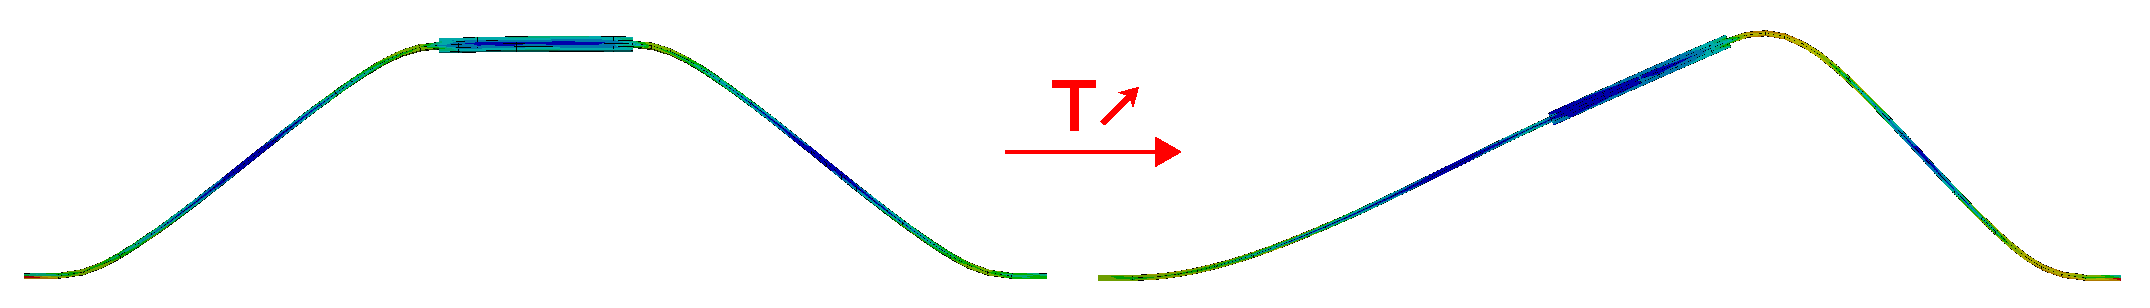
\includegraphics[width=\textwidth]{Figures/FigCentBumpTransformation.eps}
  \caption{Stable positions of the buckled beam before and after heating}
  \label{fig:modechange}
\end{figure}

% \begin{figure}[H]
%     \centering
%     \begin{subfigure}[t]{0.4\textwidth}
% 			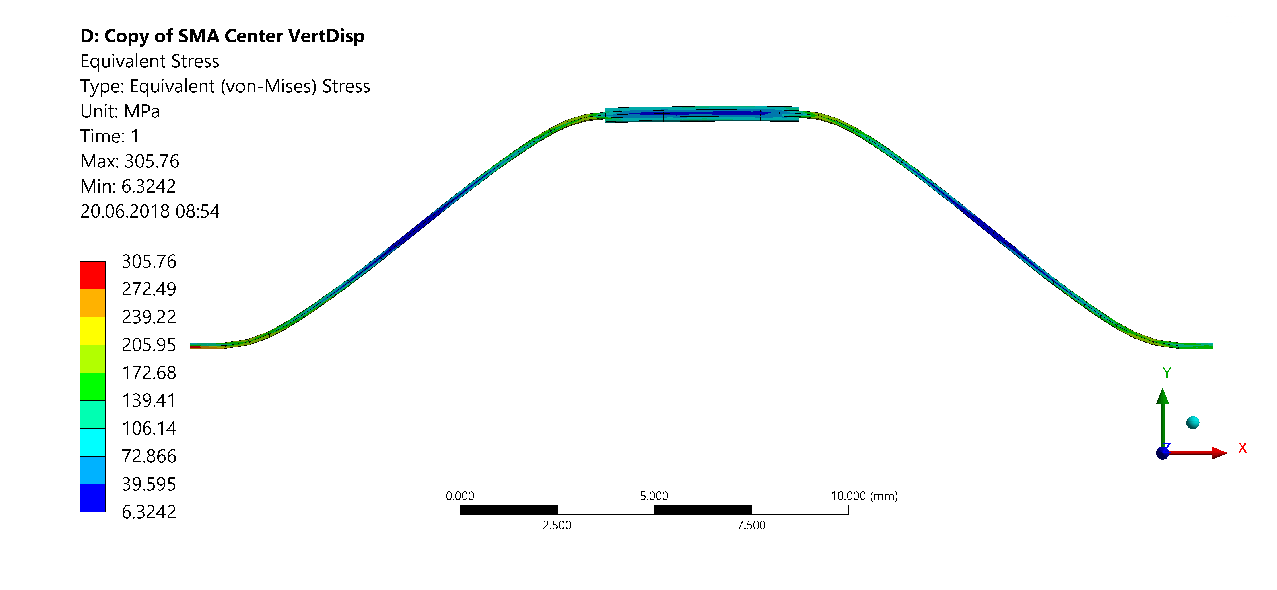
\includegraphics[width=\textwidth]{Figures/FigCentBumpBefore2x.eps}
% 			\caption{Before heating}
% 			\label{fig:modechangebefore}
%     \end{subfigure}
% 		~
%      %add desired spacing between images, e. g. ~, \quad, \qquad, \hfill etc.
%       %(or a blank line to force the subfigure onto a new line)
%     \begin{subfigure}[t]{0.4\textwidth}
% 			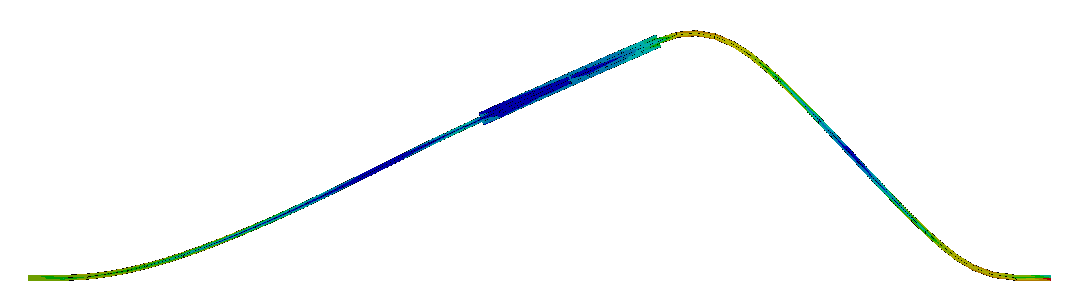
\includegraphics[width=\textwidth]{Figures/FigCentBumpAfter2x.eps}
% 			\caption{After heating}
% 			\label{fig:modechangeafter}
%     \end{subfigure}
% 		\caption{Stable positions of the buckled beam}
% 		\label{fig:modechange}
% \end{figure}

The direction in which the blade transitions is due to the convergence of the solution in the simulation. In an experimental scenario, the direction of the transformation can be controlled by creating an asymmetry in the thermal load or mechanical conditions. By applying a thermal load to either direction, the direction of the final stable mode can be chosen.

\subsection{Test bench layout}
So as to study the thermal properties of the SMA blade, a test bench that was designed to measure the time response of the SMA actuator is constructed as shown in figure~\ref{fig:test_bench}.
\newpage
% \begin{figure}[H]
%   \centering
%   \begin{subfigure}[b]{0.45\textwidth}
%     {\footnotesize
%     \def\svgwidth{\columnwidth}
%     \input{Figures/Test_Bench_Sample_Refactor.pdf_tex}
%     }
%     \caption{Layout of the test bench and examples of SMA blade samples generated using factors described in section \ref{ssec:WA_TRE}.}
%     % \vspace{-5pt}
%     \label{fig:test_bench}
%   \end{subfigure}
%   ~
%   %add desired spacing between images, e. g. ~, \quad, \qquad, \hfill etc.
%   %(or a blank line to force the subfigure onto a new line)
%   \begin{subfigure}[b]{0.45\textwidth}
%     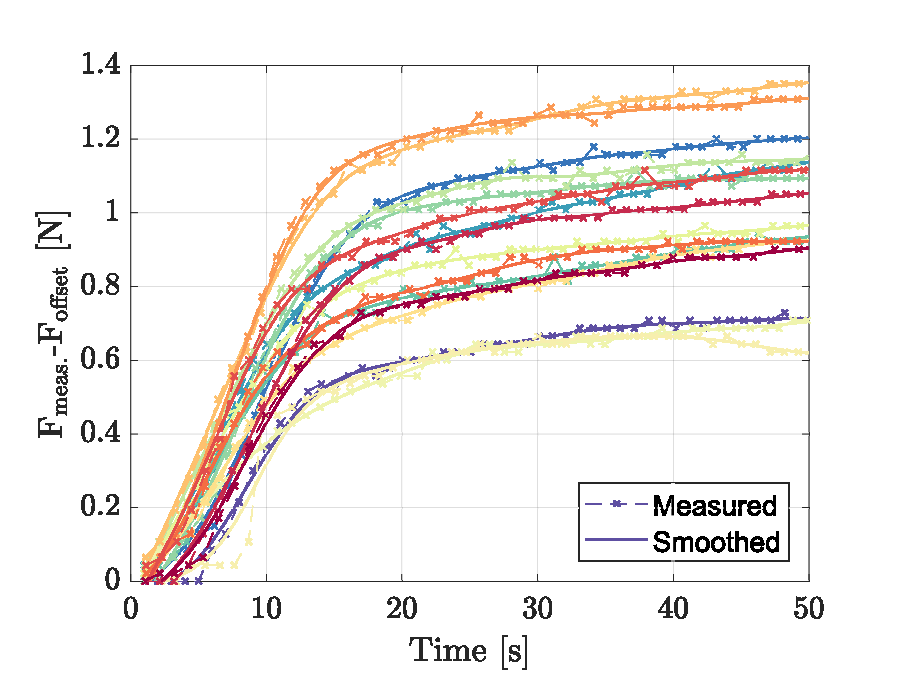
\includegraphics[width=\textwidth]{Figures/TB_Measurements.eps}
%     \caption{Force-time measurements obtained using the test bench.}
%     \label{fig:TB_Measurements}
%   \end{subfigure}
%   \caption{Representation of analytical model of buckled beam obtained from literature\cite{timoshenko_theory_1962}.}
%   \label{fig:Buckled_Beam}
% \end{figure}
\begin{wrapfigure}{r}{0.55\textwidth}
	\vspace{10pt}
	\centering
  {\footnotesize
  	\def\svgwidth{0.5\columnwidth}
  	\input{Figures/Test_Bench_Sample_Refactor.pdf_tex}
  }
	\caption{Layout of the test bench and examples of SMA blade samples generated using factors described in section \ref{ssec:WA_TRE}.}
	\vspace{-5pt}
	\label{fig:test_bench}
\end{wrapfigure}

An SMA blade is fixed between two electrodes which allow an electrical current to flow through the system. In this setup, the right electrode is part of the main body of the test bench while the left electrode is placed on a linear guide in order for it to be able to move only unidirectionally. Using this mobile part, the blade is preconstrained while in its M phase i.e. at low temperature. A force sensor is then placed behind the left electrode and fixed to the bench to measure the force applied by the SMA actuator while it tries to return to its initial shape during the transition from the M phase to the A phase, i.e. heating. The time required for the blade to reach its maximum force output can then be measured.

\subsection{Thermal response enhancement}\label{ssec:WA_TRE}
% \begin{wrapfigure}{l}{0.45\textwidth}
% 	\vspace{-10pt}
%     \centering
%     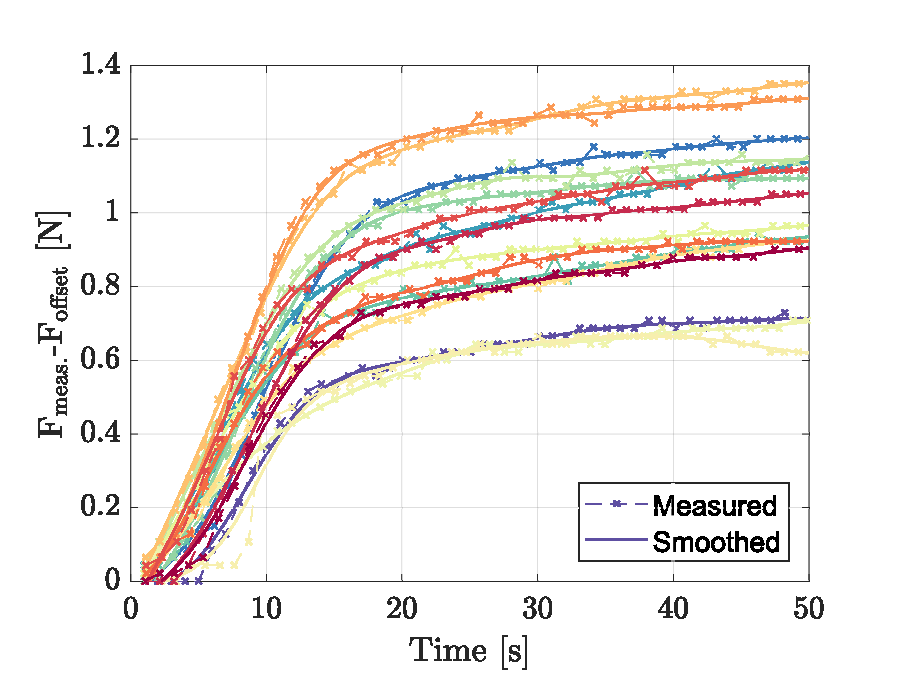
\includegraphics[width=0.45\textwidth]{Figures/TB_Measurements.eps}
%     \vspace{-20pt}
%     \caption{Force-time measurements of the d ifferent SMA blades obtained using the test bench.}
% 		\vspace{-10pt}
%     \label{fig:bar1}
% \end{wrapfigure}

This next section aims to optimise the heating of the SMA in critical sections and thus improve the force output and actuation times of the SMA actuator. The SMA blades are actuated using Joule heating where a current is passed through the blade and the internal resistance is used to heat the blade. Thus, the geometry of the blade is critical when optimizing the time response of the shape memory effect. The design of the SMA blades were created based on the location and orientation of perforations that were placed on the surface of the blade. The volume of material of the blade was also kept constant so as to have the same quantity of material to be heated during each run. This is controlled by ensuring that the thickness of blades are the same and that the total surface area is constant between each blade.

\begin{figure}[H]
  \centering
  \begin{minipage}{.45\textwidth}
    \centering
    \vspace{-10pt}
    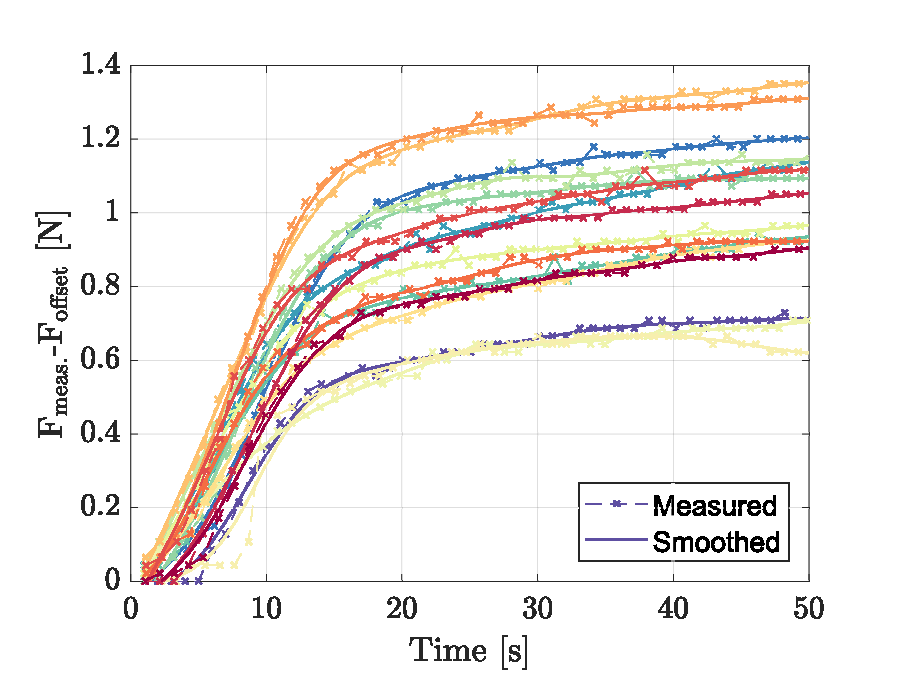
\includegraphics[width=\textwidth]{Figures/TB_Measurements.eps}
    \vspace{-20pt}
    \caption{Force-time measurements of the different SMA blades obtained using the test bench.}
		\vspace{-10pt}
    \label{fig:TB_Measurements}
  \end{minipage}%
  \hfill
  \begin{minipage}{.47\textwidth}
    \centering
    \vspace{-6pt}
    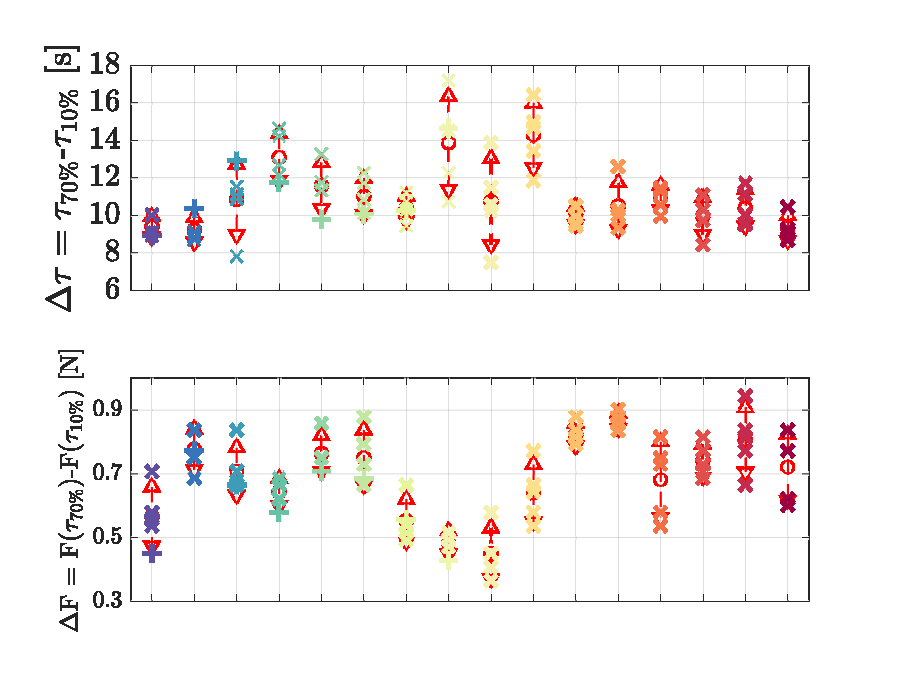
\includegraphics[width=\textwidth]{Figures/Had_RawData.eps}
    \vspace{-26pt}
    \caption{Results of the experiment conducted on the different SMA blade shapes showing the effect on the force output and the time constant.}
    \vspace{-10pt}
     \label{fig:Had_RawData}
  \end{minipage}
\end{figure}


% The design of the SMA blades was created based on four factors as defined below while also keeping the volume of material used constant:
% \begin{enumerate}[label=\textbf{~~~~Factor $x_{\arabic*}$}:,align=left]
%   \item Number of perforations along the width
%   \item Position of the holes along the length
%   \item Number of perforations along the length
%   \item Orientation of the perforation
% \end{enumerate}
The conventional option for the design of the test would be to design changes in the beam based on one factor at a time and observe the effect on the time response. This method is inefficient and time-consuming. Furthermore, the material is quite expensive, so extracting quality information for multiple construction factors from each blade is primordial. Thus, the effect of each parameter has been explored using a statistical approach based on a Hadamard matrix as presented in the work \ref{bib:TimeResponse}. This experiment performs an analysis of the factors with respect to the time response in terms of the force-time derivative while reducing the number of runs and the quantity of material used.

% \begin{wrapfigure}{r}{0.46\textwidth}
%    \vspace{-10pt}
%     \centering
%     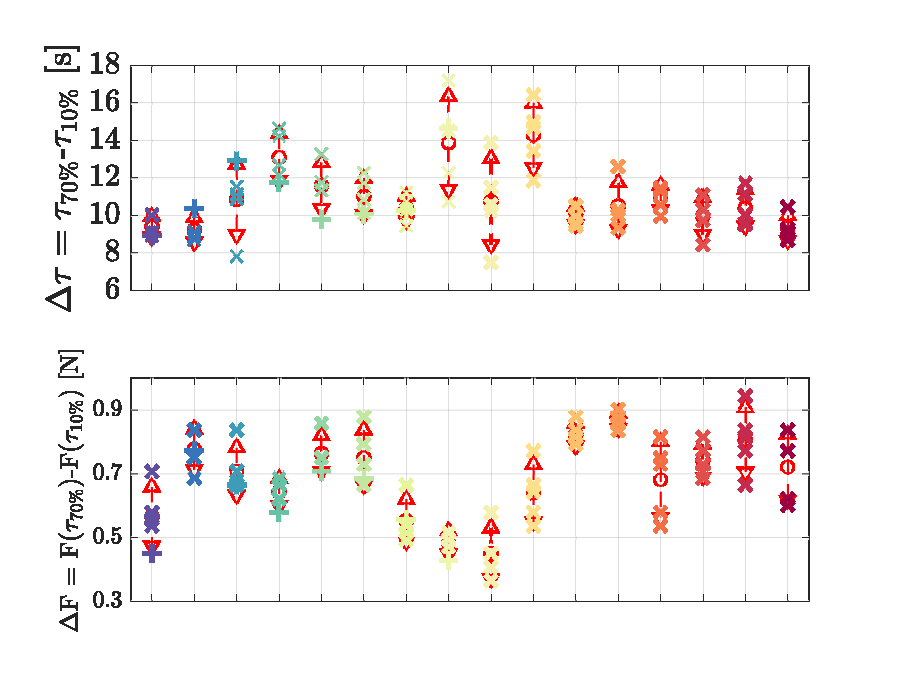
\includegraphics[width=0.5\textwidth]{Figures/Had_RawData.eps}
%     \vspace{-25pt}
%     \caption{Results of the experiment conducted on the different SMA blade shapes showing the effect on the force output and the time constant.}
% 		\vspace{-10pt}
%     \label{fig:bar1}
% \end{wrapfigure}

Here, the material used was a NiTiNOL with a low transformation temperature and thus existed mostly in the A phase at room temperature. Thus, due to a combination of ineffective power management during the heating process and the refrigeration required to observe the SME in the blade, the time response of the blades are much larger than the required use case scenario. Nevertheless, the experiment shows that the test bench can be used to create a preliminary test with the ability to measure the time response of a heated buckled SMA beam. The experiment was also able to shows that for the same quantity of material and by just changing the location of the perforations on the blade, the time responses can be improved.
% A linear fit of the force derivative with respect to time $\frac{dF}{dt}$ was performed, in the form of $\frac{dF}{dt} \sim x_1+x_2+x_3+x_4 $ (in Wilkinson notation) for the Hadamard with one run, five runs, and the full fold-over. The upper plot of figure \ref{fig:bar1} represents the influence of each factor upon the experiment with respect to the residual of this model. It is desirable to obtain coefficients whose significance is high with F-value $\geq$ 1. The lower plot represents the p-value, which is the probability of having validated a hypothesis by chance. In this case, the hypothesis is that factors have a non-zero influence in the model; meaning that small p-values (being sure that the parameters have a non-null influence) are desirable. It was deemed that concluding results should have p-values $\leq$ 0.05. Given their corresponding p-values, it could be affirmed that the factors $x_2$, $x_3$ and $x_4$ indeed affect the force vs time of the SMA blade; the longitudinal centring of the perforations, the number of them and their orientation, respectively.

The work \ref{bib:TimeResponse} shows that the effective use of power in the SMA blade can lead to better output forces and better time responses. The response of a SMA blade in terms of maximal force-time derivative can be optimised by carefully placed perforations. Indeed, an improvement by a factor of 3 could be observed between the highest and the lowest response in this experiment using the same quantity of material. This technique could be used in combination with the buckled SMA beam to efficiently heat the appropriate regions of the blade and eventually create a self-switching SMA actuator. The perforations create zones of higher resistance and thus more effective heating. This same principle can be used to find the appropriate areas to place printed coil heaters to further optimize the time response of the SMA actuator.

\section{Originality of the Research} \label{sec:originality}
The originality of this work lies in the pursuit of designing a gripper system that can harness the high work output of shape memory alloys. The gripper will be inspired by the various innovative smart technology explored within the state of the art. The state of the art shows that there exists many novel ideas for compact, light weight actuators using smart materials but non that are capable of delivering the high work output seen in SMAs. By harnessing the strengths of the SMA and the innovative strategies used in other smart material actuator systems, this research aims to explore the capabilities of the SMA material and develop an innovative gripper system. The following topics are expected to be studied over the course of this research project :
\begin{enumerate}
  \item Investigation of the SMA capabilities through the study of an analytical and finite element model
  \item Optimization of the topology of the active material component in the system for increased performances
  \item Optimization of heating and cooling strategies of the SMA so as to decrease response times and bandwidth
  \item Design and integration of a bistable system that incorporates an active smart material such as an SMA to achieve a responsive and powerful gripper system
\end{enumerate}

% \section{Thesis Plan}
The following list presents a non-definitive thesis plan :
\begin{enumerate}
  \item Motivation of the Thesis
  \item State of the art : smart materials and actuation structures
  \item Integration of SMAs into bistable systems
  \item Enhancement of deposition techniques for electrodes and time response \todo{Reformulate this step}
  % \item Control
  \item Prototyping and validation
  \item Conclusion
\end{enumerate}

% \section{Gantt Diagram}\label{sec:gantt}
\vspace{-1mm}
The follow diagram proposes a 4-year course for the doctorate. Some relevant conferences are displayed within the diagram.
%%PATO SUGGESTION
\begin{figure}[H]
\centering
\begin{ganttchart}
[
vgrid,
hgrid,
today=4,
newline shortcut=true,
bar label node/.append style={align=right},
x unit=.7 cm,
y unit chart=.4 cm,
today rule/.style={draw=tableRed, ultra thick},
milestone/.append style={fill=Goldenrod,rounded corners=.5pt,style={xscale=0.3}}%,
%milestone left shift=-.2,
]{1}{16}
\gantttitle{\footnotesize{2017}}{1}
\gantttitle{2018}{4}
\gantttitle{2019}{4}
\gantttitle{2020}{4}
\gantttitle{2021}{3} \\
%%%CTI
%\ganttbar[bar/.append style={fill=magenta}]{Modelling Bearingless}{1}{3}\\
%\ganttbar[bar/.append style={fill=magenta}]{Conception and Optimization}{3}{6}\\
%\ganttbar[bar/.append style={fill=magenta}]{Realization of Ventilation Prototype}{6}{8}\\
%\ganttbar[bar/.append style={fill=magenta}]{Command Electronics}{8}{10}
%%%
%\ganttnewline[thick, blue]
\ganttbar[
bar/.append style={fill=color1}
]{\footnotesize{Literature Review}}{1}{2}\\

\ganttbar[
bar/.append style={fill=color1}
]{\footnotesize{Modeling of SMAs}}{2}{3}

\ganttmilestone[
inline, milestone inline label node/.append style={right=1mm},
milestone/.append style={fill=greenColor3},
milestone left shift=.4,
milestone right shift=.4,
]{\href{http://www.icems2018.com/}{ICEMS 18'}}{4}\\

\ganttbar[
bar/.append style={fill=color2}
]{\footnotesize{Catalogue of Bistable Solutions}}{3}{3}

\ganttmilestone[
inline, milestone inline label node/.append style={right=1mm},
milestone/.append style={fill=greenColor3},
milestone left shift=.6,
milestone right shift=.6,
]{\href{http://www.icems2018.com/}{ICEMS 18'}}{4}\\

\ganttbar[bar/.append style={fill=color2}]{\footnotesize{FEM Analysis of Systems}}{3}{4}

\ganttmilestone[
inline, milestone inline label node/.append style={right=1mm},
milestone/.append style={fill=greenColor1},
milestone left shift=.0,
milestone right shift=.0,
]{\href{https://ldia2019.epfl.ch/}{LDIA 19'}}{6}\\

%\ganttmilestone[inline]{ICEMS}{5}\\
\ganttbar[
bar/.append style={fill=color3}
]{\footnotesize{Time Response Enhancement}}{3}{6}

\ganttmilestone[
inline, milestone inline label node/.append style={right=1mm},
milestone/.append style={fill=greenColor1},
milestone left shift=.0,
milestone right shift=.0,
]{\href{http://www.aim2019.org/}{AIM 19'}}{8}\\

\ganttbar[
bar/.append style={fill=color3}
]{\footnotesize{SMA Integration Analysis}}{6}{8}\\

\ganttbar[
bar/.append style={fill=color3}
]{\footnotesize{Electrode Deposition Analysis}}{8}{9}\\

\ganttbar[
bar/.append style={fill=color4}
]{\footnotesize{1$^{\text{st.}}$ Prototype}}{10}{12}\\

% \ganttmilestone[
% inline, milestone inline label node/.append style={right=1mm},
% milestone left shift=.0,
% milestone right shift=.0,
% ]{\href{https://ias.ieee.org/events-conferences/conference-schedule.html}{APEC 20'}}{12}\\

\ganttbar[
bar/.append style={fill=color4}
]{\footnotesize{Prototyping and Validation}}{12}{14}\\

\ganttbar[bar/.append style={fill=color5}]{\footnotesize{Redaction}}{15}{16}
\end{ganttchart}
\label{fig:gantt}
\vspace{-10mm}
\end{figure}

% \section{Publications}
{\small
\begin{enumerate}[label={[\Alph*]}]
  \item \emph{Accepted:} S. Thomas, M. Almanza, Y. Civet, and Y. Perriard, ``Actuation Displacement Analysis of a Self-Switching Shape Memory Alloy Buckled Beam'', in \emph{IEEE International Conference on Electrical Machines and Systems}, Jeju, 2018, p. 7. \label{bib:SelfSwitch}
  \item \emph{Accepted:} S. Thomas, P. Peralta, R. Mottet, M. Lehmann, Y. Civet, and Y. Perriard, ``Analysis and Reduction of Time Response in Thermally Activated Shape Memory Alloys'', in \emph{IEEE International Conference on Electrical Machines and Systems}, Jeju, 2018, p. 6. \label{bib:TimeResponse}
\end{enumerate}
}


%\printbibliography[heading=bibintoc]
%\label{bib:mybiblio}
%\section*{Problem Statement}
%Put your Problem statement here! Example of a Citation\cite[p.219]{Robotics}. Here's Another Citation\cite{Flueck}
%
%\section*{Investigation/Research}
%\lipsum[2]
%
%\section*{Alternative Solutions}
%\lipsum[3]
%
%\section*{Optimum Solution}
%\lipsum[4]
%% to comment sections out, use the command \ifx and \fi. Use this technique when writing your pre lab. For example, to comment something out I would do:
%%  \ifx
%%	\begin{itemize}
%%		\item item1
%%		\item item2
%%	\end{itemize}
%%  \fi
%
%\section*{Construction/Implementation}
%\lipsum[5]
%
%\section*{Analysis \& Testing}
%\lipsum[6]
%
%\section*{Final Evaluation}
%\lipsum[7]
%
%\section*{Attachments}
%%Make sure to change these
%Lab Notes, HelloWorld.ic, FooBar.ic
%%\fi %comment me out
%
%\begin{thebibliography}{9}
%\bibitem{Robotics} Fred G. Martin \emph{Robotics Explorations: A Hands-On Introduction to Engineering}. New Jersey: Prentice Hall.
%\bibitem{Flueck}  Flueck, Alexander J. 2005. \emph{ECE 100}[online]. Chicago: Illinois Institute of Technology, Electrical and Computer Engineering Department, 2005 [cited 30
%August 2005]. Available from World Wide Web: (http://www.ece.iit.edu/~flueck/ece100).
%\end{thebibliography}
\bibliographystyle{ieeetr}
\bibliography{Candidacy_ST_RevB}

\end{document}
